% !TEX encoding = UTF-8
% !TEX TS-program = pdflatex
% !TEX root = ../tesi.tex
% !TEX spellcheck = it-IT

%*************************************************************
\chapter{Tecnologie utilizzate}
\label{cap:tecnologie-utilizzate}
%*************************************************************

La tecnologia principale con cui viene effettuata la stima della distanza è la tecnologia BLE. La tecnologia BLE è presente sia sui TAG, dislocati nell'ambiente indoor, sia sullo smartphone, usato per identificare la risorsa in movimento. Per lo sviluppo dell'applicazione sullo smartphone si è analizzata la struttura del sistema Android per poi implementare l'applicazione in linguaggio Java. La scelta dei protocolli da utilizzare a livello applicativo è ricaduta su HTTP, per le comunicazioni effettuate attraverso l'interfaccia web, e MQTT, per le comunicazioni effettuate attraverso lo smartphone Android. I fattori che hanno portato a scegliere MQTT, rispetto ad altri protocolli, sono la leggerezza e l'affidabilità oltre al fatto di essere uno standard definito e aperto.

Per lo sviluppo dei vari componenti si è utilizzato Node.js, runtime Javascript costruito sul motore JavaScript V8 di Google Chrome.

I database utilizzati per la memorizzazione dei dati sono di tipo relazionale e in particolare si è utilizzato SQLite per la memorizzazione dei dati nel sistema Android mentre si è utilizzato Microsoft SQL Server per la memorizzazione delle posizioni di tutte le risorse.

Dato che si sono utilizzati database relazionali, SQLite per Android e Microsoft SQL Server per la gestione della persistenza del sistema, per le interrogazioni si utilizza il linguaggio SQL.

Per l'applicazione web si è scelto l'approccio \emph{Single Page Application} con il fine di favorire l'interattività. Per realizzare l'interfaccia web si sono utilizzate diverse tecnologie, quali: HTML, CSS, AJAX, Canvas.

Il formato comune utilizzato per l'interscambio dei dati tra i vari componenti è il JSON.

Di seguito si descrivono brevemente le varie tecnologie utilizzate.

\section{Bluetooth}
Nelle telecomunicazioni, Bluetooth \cite{wiki:bluetooth} è uno standard tecnico-industriale di trasmissione dati per reti personali senza fili. Fornisce un metodo standard, economico e sicuro per scambiare informazioni tra dispositivi diversi attraverso una frequenza radio sicura a corto raggio.
La specifica Bluetooth è stata sviluppata da Ericsson e in seguito formalizzata dalla Bluetooth Special Interest Group (SIG). Il protocollo Bluetooth opera nel campo di frequenze assegnato intorno ai 2,45 GHz. Per ridurre le interferenze il protocollo divide la banda in 79 canali e provvede a commutare tra i vari canali 1.600 volte al secondo (frequency hopping).

Nel corso degli anni sono state emesse diverse versioni del protocollo ognuna delle quali implementa diverse specifiche. Ogni dispositivo Bluetooth è configurabile per cercare costantemente altri dispositivi e per collegarsi a questi.

\subsection{Bluetooth 4.0 e BLE}
In data 6 luglio 2010 sono diventate definitive le specifiche della versione 4.0.

Rispetto alle versioni precedenti, la versione 4.0 punta alla riduzione dei consumi energetici. L'obiettivo principale di questa funzionalità opzionale, denominato Low Energy (LE), tramite un'ottimizzazione della struttura di trama e l'impiego di dispositivi più efficienti, comporta una riduzione della velocità, che in questa modalità si attesta a 1 Mbps. In termini trasmissivi, sono stati potenziati i meccanismi di rilevazione e correzione di errore e di cifratura del segnale col supporto di AES-128.

\subsection{TAG BLE}
Un TAG BLE \cite{globaltag:tagble} è un beacon BLE che può contenere, inoltre, un accelerometro, un sensore di temperatura e di umidità. In figura \ref{fig:tag-ble} è possibile vedere com'è fatto un TAG BLE commercializzato da Global Tag.

Un TAG BLE dispone di un pulsante ON/OFF che consente di attivare o disattivare il tag, al fine di permettere all’utente di risparmiare la batteria, qualora non abbia la necessità di mantenere il tag acceso. La distanza di lettura arriva fino a 90 metri. I diversi parametri del beacon BLE, come l’intervallo di emissione, la potenza del segnale, il ``friendly name'' si possono configurare tramite software.

\begin{figure}[htp]
	\centering
	\includegraphics[height=\textheight/3]{tag-ble}
	\caption{TAG BLE}
	\label{fig:tag-ble}
\end{figure}

\section{Il sistema Android}
Android \cite{android:site} è un sistema operativo per dispositivi mobili sviluppato da Google Inc. basato sul kernel Linux. È un sistema embedded progettato principalmente per smartphone e tablet.

Lo sviluppo di Android prosegue attraverso l'Android Open Source Project il quale è software libero ad esclusione di diversi firmware non-liberi inclusi per i produttori di dispositivi e delle cosiddette ``Google Apps'' come ad esempio Google Play. È distribuito sotto i termini della licenza libera Apache 2.0 riservandosi di non-includere software coperto da licenze copyleft.

Android è costituito da un kernel Linux 2.6 e 3.x (da Android 4.0 in poi), con middleware, Librerie e API scritte in C (o C++) e software in esecuzione su un framework di applicazioni che include librerie Java compatibili con librerie basate su Apache Harmony.

La piattaforma hardware principale di Android è l'architettura ARM mentre le applicazioni Android sono Java-based. L'architettura software del sistema Android è schematizzata in figura \ref{fig:architettura-android}.

\begin{figure}[htp]
	\centering
	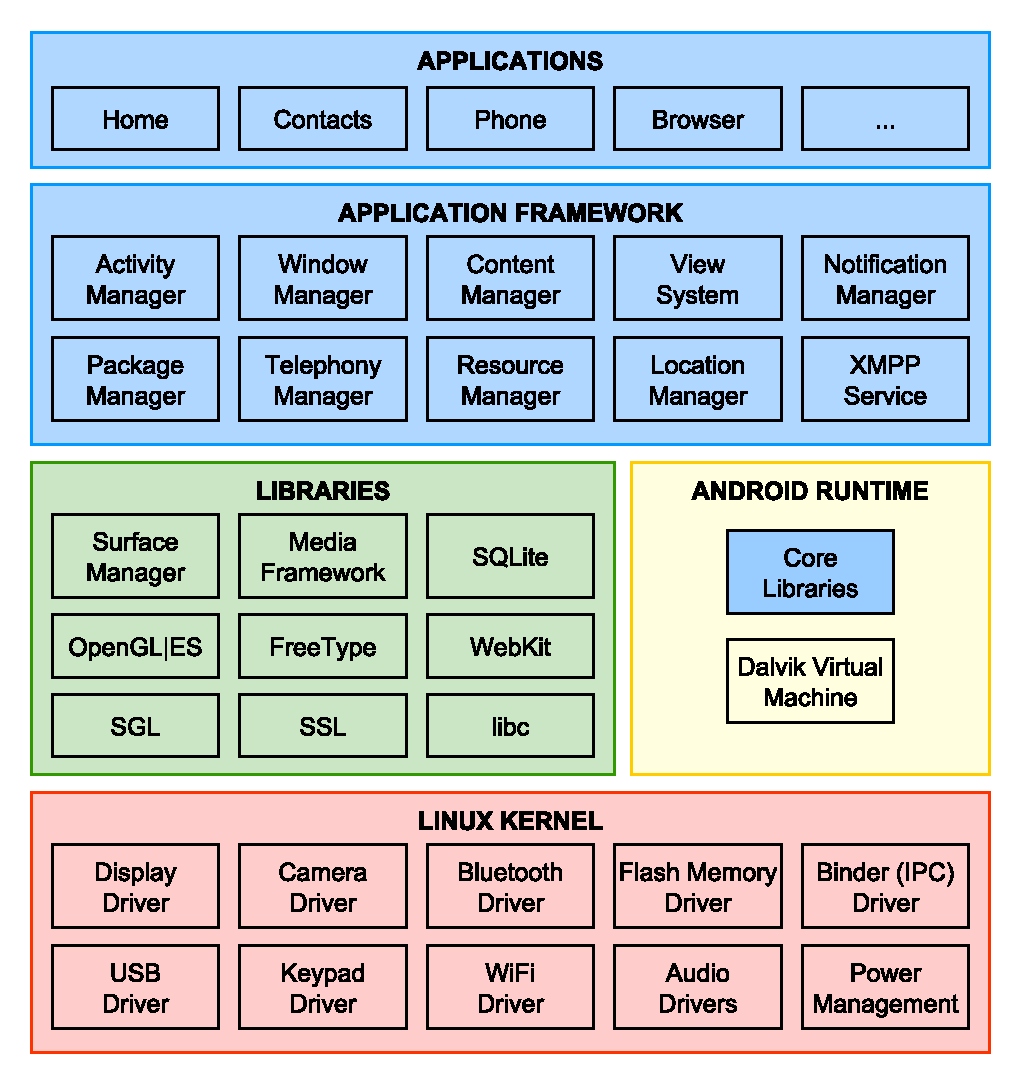
\includegraphics[height=\textheight/3]{architettura-android}
	\caption{Architettura del sistema Android}
	\label{fig:architettura-android}
\end{figure}

\section{Protocolli}

\subsection{MQTT}
MQ Telemetry Transport (MQTT) \cite{mqtt:site} è un protocollo ISO standard di messaggistica leggero di tipo publish-subscribe posizionato in cima a TCP/IP. Il protocollo è stato inventato da Andy Stanford-Clark di IBM, e Arlen Nipper di Cirrus Link Solutions nel 1999.

MQTT è stato progettato per avere bassa latenza, messaggistica sicura su reti fragili e una  distribuzione efficiente a uno o più ricevitori. Il protocollo si concentra sulla riduzione al minimo della quantità di byte necessari per l’invio del messaggio e sul basso consumo energetico. La dimensione massima dei messaggi di 256 mb, quindi non è possibile inviare per ogni messaggio grandi quantità di dati ma è possibile inviare un numero elevato di messaggi di dimensioni ridotte. MQTT fornisce, inoltre, un canale di comunicazione bidirezionale. Questo protocollo viene utilizzato in situazioni in cui è richiesto un basso impatto e dove la banda è limitata. Per poter essere utilizzato il pattern publish-subscribe richiede un \emph{message broker} il quale è responsabile della distribuzione dei messaggi ai client destinatari.

\subsection{HTTP}
L'HyperText Transfer Protocol (HTTP) \cite{HTTP:site} è un protocollo a livello applicativo usato come principale sistema per la trasmissione d'informazioni sul web ovvero in un'architettura tipica client-server. Le specifiche del protocollo sono gestite dal World Wide Web Consortium (W3C). Un server HTTP generalmente resta in ascolto delle richieste dei client sulla porta 80 usando il protocollo TCP a livello di trasporto.
Nell'HTTP le connessioni vengono generalmente chiuse una volta che una particolare richiesta, o una serie di richieste correlate, è stata soddisfatta.

\subsection{MQTT vs HTTP}
Uno dei fattori per cui si è scelto MQTT nell’applicazione Android è dato dal minor consumo di batteria e alla maggiore leggerezza ed affidabilità nella connessione. In tabella \ref{tab:https-vs-mqtt} vengono riportati i risultati di un test \cite{nicholas:https-vs-mqtt} di spedizione di 1024 messaggi con payload di 1 byte. Come si può notare dai dati in tabella utilizzando MQTT si ha una totale consegna dei messaggi inviati oltre avere un consumo di batteria inferiore per ogni messaggio inviato rispetto ad HTTPS.

\begin{table}
	\caption{Test di spedizione di 1024 messaggi con payload da 1 byte con HTTPS e MQTT}
	\label{tab:https-vs-mqtt}
	\begin{center}
		\begin{tabular}{lcccc}
			\toprule
			\textbf{Connessione} 				& \multicolumn{2}{c}{3G} & \multicolumn{2}{c}{Wifi} \\
			\midrule
			\textbf{Protocollo} 				& HTTPS 		& MQTT 			& HTTPS 		& MQTT \\
			\midrule
			\textbf{\% Batteria / Ora} 			& 18.43\% 		& 16.13\% 		& 3.45\% 		& 4.23\% \\
			\textbf{Messaggi / Ora} 			& 1708 			& 160278 		& 3628 			& 263314 \\
			\textbf{\% Batteria / Messaggio} 	& 0.01709 		& 0.00010 		& 0.00095		& 0.00002 \\
			\textbf{Messaggi Ricevuti} 			& 240/1024 		& 1024/1024 	& 524/1024 		& 1024/1024 \\
			\bottomrule
		\end{tabular}
	\end{center}
\end{table}


\section{NodeJS}
Node.js \cite{node:site} è un runtime Javascript costruito sul motore JavaScript V8 di Google Chrome. Il modello utilizzato da Node.js è il modello I/O non bloccante ad eventi, che lo rende un framework leggero ed efficiente. Il modello I/O non bloccante richiede al sistema operativo di ricevere notifiche al verificarsi di determinati eventi, rimanendo quindi in sleep fino alla notifica stessa. Quando la notifica avviene, allora il sistema operativo torna attivo per eseguire le istruzioni previste nella funzione di callback, funzione che viene eseguita una volta che il risultato dell'elaborazione da parte del sistema operativo è disponibile.

Node.js è organizzato in moduli i quali sono scritti in JavaScript. Ogni sviluppatore può scrivere nuovi moduli in JavaScript oppure può includere dei moduli già scritti prelevandoli da npm, gestore dei pacchetti predefinito di Node.js.

\section{JavaScript}
JavaScript \cite{javascript:site} è un linguaggio di scripting orientato agli oggetti e agli eventi, comunemente utilizzato nella programmazione Web lato client per la creazione, in siti web e applicazioni web, di effetti dinamici interattivi tramite funzioni di script invocate da eventi innescati a loro volta in vari modi dall'utente sulla pagina web in uso. Tali funzioni di script, utilizzati dunque nella logica di presentazione, possono essere opportunamente inserite in file HTML. JavaScript è stato standardizzato per la prima volta il 1997 dalla ECMA con il nome ECMAScript ed è, inoltre, uno standard ISO.

\section{SQL}
SQL (Structured Query Language) \cite{wiki:sql} è un linguaggio standardizzato per database basati sul modello relazionale (RDBMS) progettato per:
\begin{itemize}
	
	\item Creare e modificare schemi di database (Data Definition Language);
	
	\item Inserire, modificare e gestire dati memorizzati (Data Manipulation Language);
	
	\item Interrogare i dati memorizzati (Data Query Language);
	
	\item Creare e gestire strumenti di controllo ed accesso ai dati (Data Control Language).
	
\end{itemize}
SQL non è solo di un semplice linguaggio di interrogazione, ma alcuni suoi sottoinsiemi si occupano della creazione, della gestione e dell'amministrazione del database.

\section{Single Page Application}
Con Single Page Application \cite{wiki:single-page-application} si intende un'applicazione web che può essere usata o consultata su una singola pagina web con l'obiettivo di fornire un'esperienza utente più fluida, simile alle applicazioni desktop dei sistemi operativi tradizionali. In un'applicazione su singola pagina tutto il codice necessario è recuperato in un singolo caricamento della pagina mentre le risorse appropriate sono caricate dinamicamente e aggiunte alla pagina quando necessario, di solito in risposta ad azioni dell'utente. In particolare, la pagina non si ricarica in nessun punto del processo, né lascia il controllo a un'altra pagina. Di seguito si presentano brevemente le tecnologie con cui si sviluppa un'applicazione web di questo tipo.

\subsection{HTML}
L'HTML (HyperText Markup Language) \cite{HTML:site} è un linguaggio di markup. Nato per la formattazione e impaginazione di documenti ipertestuali disponibili nel web 1.0, oggi è utilizzato principalmente per il disaccoppiamento della struttura logica di una pagina web. L'HTML è un linguaggio di pubblico dominio, la cui sintassi è stabilita dal World Wide Web Consortium (W3C). È derivato da SGML, un metalinguaggio finalizzato alla definizione di linguaggi utilizzabili per la stesura di documenti destinati alla trasmissione in formato elettronico.

\subsection{CSS}
Il CSS (Cascading Style Sheets) \cite{CSS:site} è un linguaggio usato per definire la formattazione di documenti HTML, XHTML e XML. L'introduzione del CSS si è resa necessaria per separare i contenuti delle pagine HTML dalla loro formattazione e permettere una programmazione più chiara e facile da utilizzare, sia per gli autori delle pagine stesse sia per gli utenti, garantendo contemporaneamente anche il riutilizzo di codice e una sua più facile manutenzione.

\subsection{AJAX}
AJAX (Asynchronous JavaScript and XML) \cite{AJAX:site} è una tecnica di sviluppo software per la realizzazione di applicazioni web interattive. Lo sviluppo di applicazioni HTML con AJAX si basa su uno scambio di dati in background fra web browser e server, che consente l'aggiornamento dinamico di una pagina web senza esplicito ricaricamento da parte dell'utente. AJAX è asincrono nel senso che i dati extra sono richiesti al server e caricati in background senza interferire con il comportamento della pagina esistente. Normalmente le funzioni richiamate sono scritte con il linguaggio JavaScript. Tuttavia, l'uso di JavaScript e di XML non è obbligatorio, come non è detto che le richieste di caricamento debbano essere necessariamente asincrone.

\section{JSON}
JSON (JavaScript Object Notation) \cite{json:site} è un formato adatto all'interscambio di dati fra applicazioni client-server. È basato sul linguaggio JavaScript Standard ECMA-262 3\ap{a} edizione dicembre 1999, ma ne è indipendente. Viene usato in AJAX come alternativa a XML/XSLT.